\documentclass[../thesis.tex]{subfiles}

\begin{document}

\chapter{The Daya Bay experiment}
\label{chap:experim}

\section*{Introduction}

The Daya Bay experiment was designed to measure $\theta_{13}$ by observing the
antineutrinos produced by the six 2.9~GW$_{\text{th}}$ nuclear reactors of the
Daya Bay and Ling Ao power plants, located near Shenzhen in southern China. A
total of eight functionally identical antineutrino detectors (ADs) were
deployed, each containing a target of 20~tons of gadolinium-doped liquid
scintillator (GdLS). Four of the ADs were evenly divided among two near halls
($\sim$350-600~m baselines from the cores), and the remaining four were placed
in a single far hall ($\sim$1500-1950~m baselines). Shielding from cosmic rays
was provided by $\sim$100~m and $\sim$300~m, respectively, of mountainous
overburden at the near and far halls. The ADs in each hall were immersed in
instrumented water pools which provided shielding from ambient radioactivity and
detection of Cerenkov radiation from atmospheric muons. Redundant detection of
muons, as well as directional information, were made available by resistive
plate chambers (RPCs) laid on top of the water pools. In this chapter we discuss
further details of the layout, the detectors, and the shielding and vetoing
system of the experiment.

\section{Site layout}
\label{sec:expLayout}

\begin{figure}[ht]
  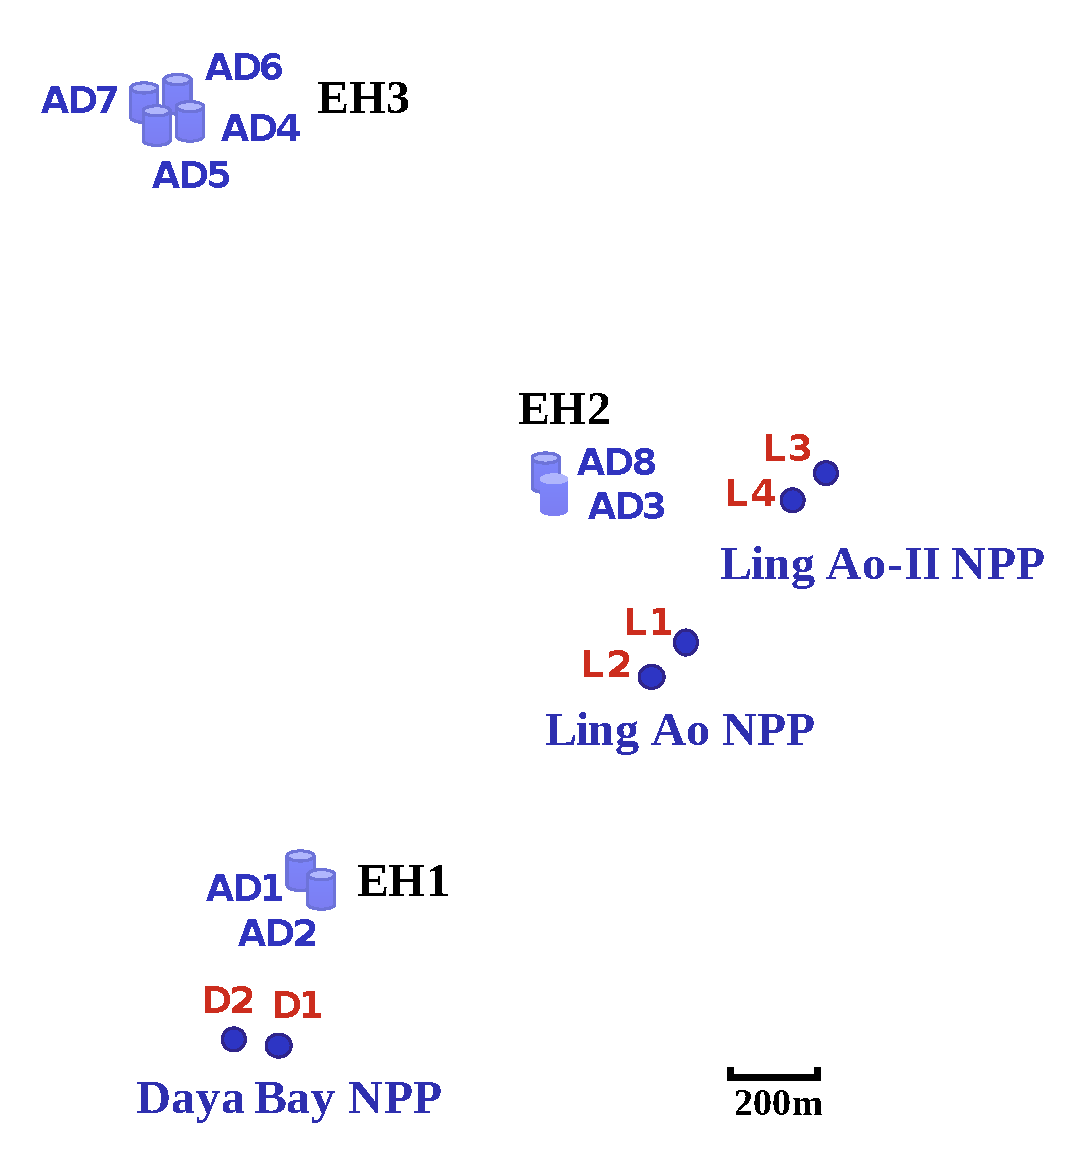
\includegraphics[scale=0.4]{inkLayout.pdf}
  \caption{The layout of the Daya Bay experiment. Modified from
    \cite{SideBySide}.}
  \label{fig:layout}
\end{figure}

As shown in \autoref{fig:layout}, the power reactors are divided into three
nuclear power plants (NPPs) of two cores each. One of the two clusters contains
the Daya Bay NPP (cores D1 and D2), while the other cluster consists of the Ling
Ao (L1 and L2) and Ling Ao-II (L3 and L4) NPPs. EH1 is located around 350~m from
the Daya Bay NPP, while EH2 is roughly 500~m from the two Ling Ao NPPs. The far
hall, EH3, in turn is located about 1900~m from the Daya Bay NPP and 1500~m from
the Ling Ao NPPs. The measured baselines, as determined from a combined GPS and
total station theodolite survey, are given in \autoref{tab:expBaselines}. The
uncertainty of $\sim$2~cm in these measurements was shown to have negligible
impact on the analysis; likewise, reactor simulations determined that the
centroid of $\nubar_e$ emission to be within $\sim$2~cm of each core's
center. Although $\nubar_e$ emission was distributed across the $\sim$3~m-scale
volume of each core, the analysis treats each core as a point source, given that
these geometric effects are negligible at Daya Bay's baselines.

\begin{table}[ht]
  \begin{tabular}{lcrrrrrr}
    \toprule
    \multicolumn{2}{c}{} & \multicolumn{6}{c}{Reactor baseline [m]} \\
    \cmidrule{3-8}
    Hall & Detector & \multicolumn{1}{c}{D1} & \multicolumn{1}{c}{D2} & \multicolumn{1}{c}{L1} & \multicolumn{1}{c}{L2} & \multicolumn{1}{c}{L3} & \multicolumn{1}{c}{L4} \\
    \midrule
    EH1  & AD1      & 362.38  & 371.76  & 903.47  & 817.16  & 1353.62 & 1265.32 \\
                         & AD2      & 357.94  & 368.41  & 903.35  & 816.90  & 1354.23 & 1265.89 \\
    EH2  & AD3      & 1332.48 & 1358.15 & 467.57  & 489.58  & 557.58  & 499.21  \\
                         & AD8      & 1337.43 & 1362.88 & 472.97  & 495.35  & 558.71  & 501.07  \\
    EH3  & AD4      & 1919.63 & 1894.34 & 1533.18 & 1533.63 & 1551.38 & 1524.94 \\
                         & AD5      & 1917.52 & 1891.98 & 1534.92 & 1535.03 & 1554.77 & 1528.05 \\
                         & AD6      & 1925.26 & 1899.86 & 1538.93 & 1539.47 & 1556.34 & 1530.08 \\
                         & AD7      & 1923.15 & 1897.51 & 1540.67 & 1540.87 & 1559.72 & 1533.18 \\
    \bottomrule
    % \multirow{2}{*}{EH1} & AD1 & 362.38 & 371.76 & 903.47 & 817.16 & 1353.62 &
    % 1265.32 \\
  \end{tabular}
  \caption{Baselines between geometric centers of the ADs and of the reactor
    cores. From \cite{An_2017}.}
  \label{tab:expBaselines}
\end{table}

\section{Antineutrino detectors}
\label{sec:expADs}

\begin{figure}[ht]
  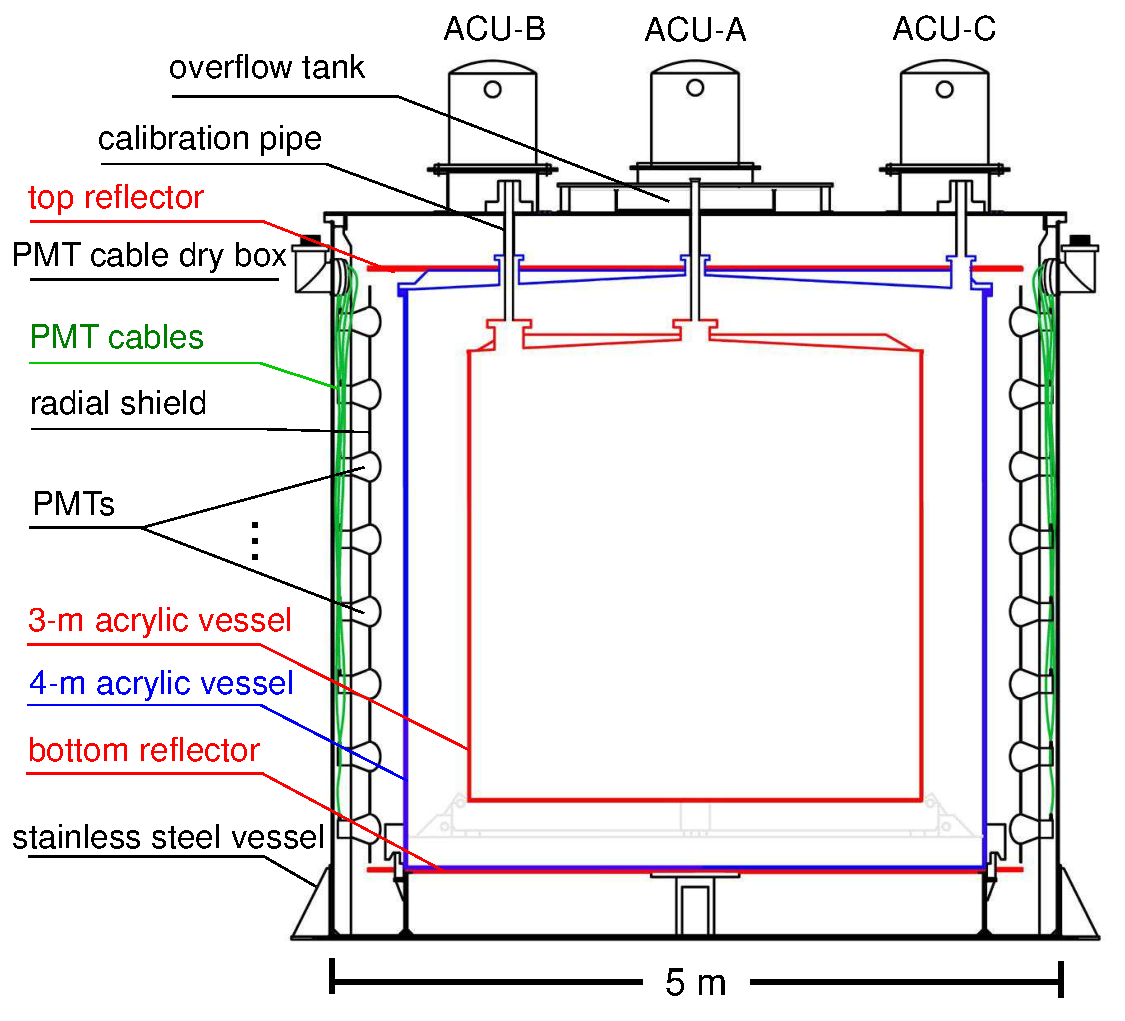
\includegraphics[scale=0.4]{exp_AD_structure.pdf}
  \caption{Structure of a Daya Bay antineutrino detector. From \cite{An_2017}.}
  \label{fig:expDetector}
\end{figure}

The design of the Daya Bay ADs is shown in \autoref{fig:expDetector}. Each AD is
made of a cylindrical stainless steel vessel (SSV), $\sim$5~m in diameter and
height, containing two nested cylinders of UV-transparent acrylic. The 3m-square
inner acrylic vessel (IAV) contains the target mass of 20~t of
GdLS\footnote{Daya Bay's liquid scintillator consists of linear alkyl benzene
  (LAB) as the solvent and medium, 3~g/L of 2,5-diphenyloxazole (PPO) as the
  fluor, and 15~mg/L of p-bis-(o-methystyril)-benzene (bis-MSB) as the
  wavelength shifter. For the GdLS, 0.1\% $^{\text{nat}}$Gd by mass was added in
  the form of a complex with 3,5,5-trimethylhexanoic acid (THMA). Further
  details can be found in \cite{Beriguete_2014}.}. Surrounding it is the
4m-square outer acrylic vessel (OAV), which contains 20~t of \emph{Gd-free}
LS. This ``gamma catcher'' volume ensures the full containment and measurement
of gammas produced near the edge of the GdLS, while also providing additional
target mass for studies (including oscillation fits) that make use of neutron
capture on hydrogen instead of on gadolinium. Between the OAV and the inner wall
of the SSV, a 37~t volume of transparent mineral oil (MO) provides shielding
from radioactivity in the detector materials, in addition to its role in
balancing the stress on the OAV wall.

Within the MO volume, the inner sidewall of the SSV supports 192 8-inch
Hamamatsu R5912 photomultipler tubes (PMTs) to detect the light from
scintillation. The PMTs are arranged in eight rings of 24 tubes whose
photocathodes protrude from matte-black radial shields that fully cover the
sidewalls, preventing light from reflecting off the walls. This simplifies the
optical characteristics of the ADs, reducing the complexity of vertex
reconstruction. Conversely, however, reflective discs are installed at the top
and bottom of the AD, improving both the energy resolution and the uniformity of
light collection versus event position. To further reduce nonuniformity effects,
each PMT is outfitted with a FINEMET conical magnetic shield to minimize
azimuthal variations in PMT response caused by the Earth's magentic field.

\subsection{PMT electronics}
\label{sec:expPmtElec}

Each PMT is positively biased via a single coaxial cable in order to achieve a
gain within 5\% of 10$^7$ (corresponding to $\sim$20 ADC counts per PE). Due to
intrinsic differences between PMTs, the necessary high voltage varies between
some 1300 to 1700~kV. Collected charge is passed through a passive decoupling
circuit which removes the HV offset; this fast ($\sim$20~ns), unbiased pulse is
then passed to the front-end electronics (FEE), where it is split and sent to
two separate circuits. One of the circuits contains a $\sim$0.25-photoelectron
(PE) discriminator, which initiates a TDC counter (of 1.6~ns resolution) to
record the presence and time of the ``hit''. The other circuit is a CR-(RC)$^4$
shaper which stretches each pulse to a length of $\sim$200~ns; the shaped pulse
is then split and sent to both a x10 ``high-gain'' amplifier and a x0.5
``low-gain'' attenuator (for neutrino-like and muon-like events, respectively)
and, finally, the two shaped and rescaled pulses are sampled by a 40~MHz 12-bit
ADC. The output of a hardware-based peak-finding algorithm is then recorded as
the raw amplitude of the pulse, for both the high-gain and low-gain
circuits. Meanwhile, the average of the four ADC samples immediately preceding
the over-threshold condition is recorded as the \emph{pre-ADC} or
\emph{pedestal} value of the hit, from which the peak ADC value is subtracted in
determining the charge, as discussed in \autoref{sec:calibGain}\footnote{The
  pre-ADC, in general, is \emph{not} taken from the four samples immediately
  preceding the \emph{peak} sample, because the peak of the shaped curve occurs
  some 100~ns after the over-threshold condition, as dictated by the time
  constant of the shaping circuit. Given the sample period of 25~ns, this
  implies a 4-5 sample lag between the over-threshold condition and the
  peak. Thus, the pre-ADC is typically taken from the average of the 5th through
  9th samples preceding the peak, give or take. This, however, changes when
  there are multiple closely-spaced hits, as illustrated later in
  \autoref{fig:closeHitsExamples}.}.

Although every hit is initially observed in this manner by the hardware, it is
only recorded in the DAQ's output stream if a trigger is issued for the AD as a
whole. An AD can be triggered both when the total observed charge is above a
software-specified threshold, as well as when the number of ``hit'' channels is
above threshold\footnote{Additional trigger types include \emph{random}
  triggers, issued at $\sim$10~Hz for monitoring of low-level activity;
  \emph{calibration} triggers, issued in sync with LED pulses during weekly
  calibrations; and \emph{cross} triggers, issued under certain conditions when
  another detector is triggered.}. Each FEE board, which reads up to 16
channels, sends two signals to the AD's \emph{local trigger board} (LTB): a
digital count of recently-hit channels (NHIT) and an analog sum of the charge
across all channels (ESUM). The LTB combines the inputs from all of the FEEs and
issues a trigger when either NHIT or ESUM are above threshold; for ordinary
physics data-taking, the thresholds are NHIT $\geq$ 45 or ESUM $\geq$ 65 pe
($\sim$0.4~MeV). When a trigger is issued, a GPS-synchronized clock (25 ns
resolution) records the overall event timestamp, each hit's TDC is stopped
(indicating the offset of each hit relative to the event timestamp), and the
readout (including the TDC, high-gain ADC, and low-gain ADC for each hit within
1.2~$\mu$s of the trigger) is sent to the DAQ system.

Thus, the raw information collected from each AD consists of a set of
triggers. Each trigger, in turn, contains a timestamp and a collection of
\emph{hits}; each hit describes the PMT ID, the TDC count, and the high- and
low-gain ADC values reported by the peak-finding circuitry. In order to be made
useful for physics analysis, the raw ADC values must first be converted into
photoelectron counts for each PMT, as described in \autoref{chap:calib}, and
then the individual PMTs must be combined and corrected to produce the amount of
energy deposited in the scintillator, as elaborated in \autoref{chap:recon}.

\subsection{Detection principle}
\label{sec:expDetPrinc}

The vast majority of events recorded by the ADs are unrelated to neutrinos. Most
events come from natural radioactivity in the detector and scintillator
materials, as well as from cosmic muons and the byproducts of muon-nucleon
reactions. Fortunately, it is possible to exploit the double-trigger nature of
neutrino events in order to effectively extract them from the data, as we
explain here.

Antineutrinos can interact with the GdLS target in a number of ways. Their
interactions can be mediated either by the $W^-$ boson (corresponding to a
\emph{charged current}, or CC, interaction), in which case the antineutrino
becomes a positron, or they can be mediated by the $Z$ boson (corresponding to a
\emph{neutral current}, or NC, interaction), in which case the antineutrino
escapes from the detector after depositing some recoil energy in the
target. Furthermore, the interaction may take place between the antineutrino and
either an electron, a proton, a neutron, or (coherently) an entire
nucleus. Among these many possibilities, however, only one channel provides a
signature that allows for efficient discrimination from background: inverse beta
decay (IBD),
\begin{equation*}
  \nubar_e + p \rightarrow e^+ + n.
\end{equation*}
This interaction is illustrated in \autoref{fig:expIBD}. An initial
\emph{prompt} scintillation signal is produced by the positron (first from
direct ionization, then from the gammas produced by annihilation). Meanwhile,
the free neutron thermalizes and is then captured by a nucleus, which quickly
de-excites, emitting gamma rays that provide a second, \emph{delayed,} signal,
closely correlated in time with the prompt signal. This ``double-pulse''
signature effectively distringuishes IBDs from events produced by natural
radioactivity, as the latter largely consists of single pulses. Meanwhile,
muon-induced double-pulse events can be eliminated by simply vetoing for a
sufficient length of time after each muon, as described in
\autoref{chap:selection}. The use of gadolinium further improves background
separation, both by reducing the neutron capture time constant from
$\sim$200~$\mu$s to $\sim$20$\mu$s, and by increasing the total energy of the
delayed gammas from 2.2 to 8~MeV. These two properties significantly reduce the
probability of accidentally identifying a pair of uncorrelated events as an IBD,
especially since the rate of uncorrelated events drops dramatically above
5~MeV. Thanks to gadolinium, such ``accidental'' backgrounds made up only 1-2\%
of the selected IBD sample. Further details regarding background measurement and
subtraction can be found in \autoref{chap:bkg}.

\begin{figure}[ht]
  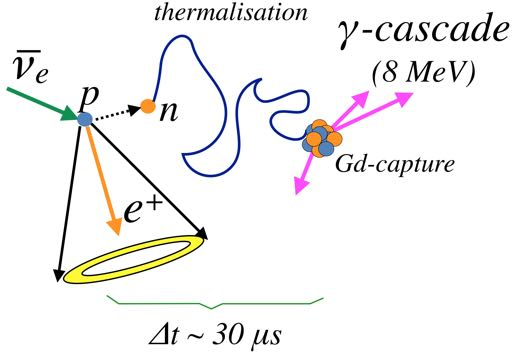
\includegraphics[scale=0.4]{ibd.png}
  \caption{An illustration of the inverse beta decay reaction. Unlike a water
    Cerenkov detector, a Daya Bay AD cannot discern the direction of the
    positron. From \cite{Fernandez_2017}.}
  \label{fig:expIBD}
\end{figure}

\section{Water pools and muon system}
\label{sec:expShieldVeto}

\begin{figure}[ht]
  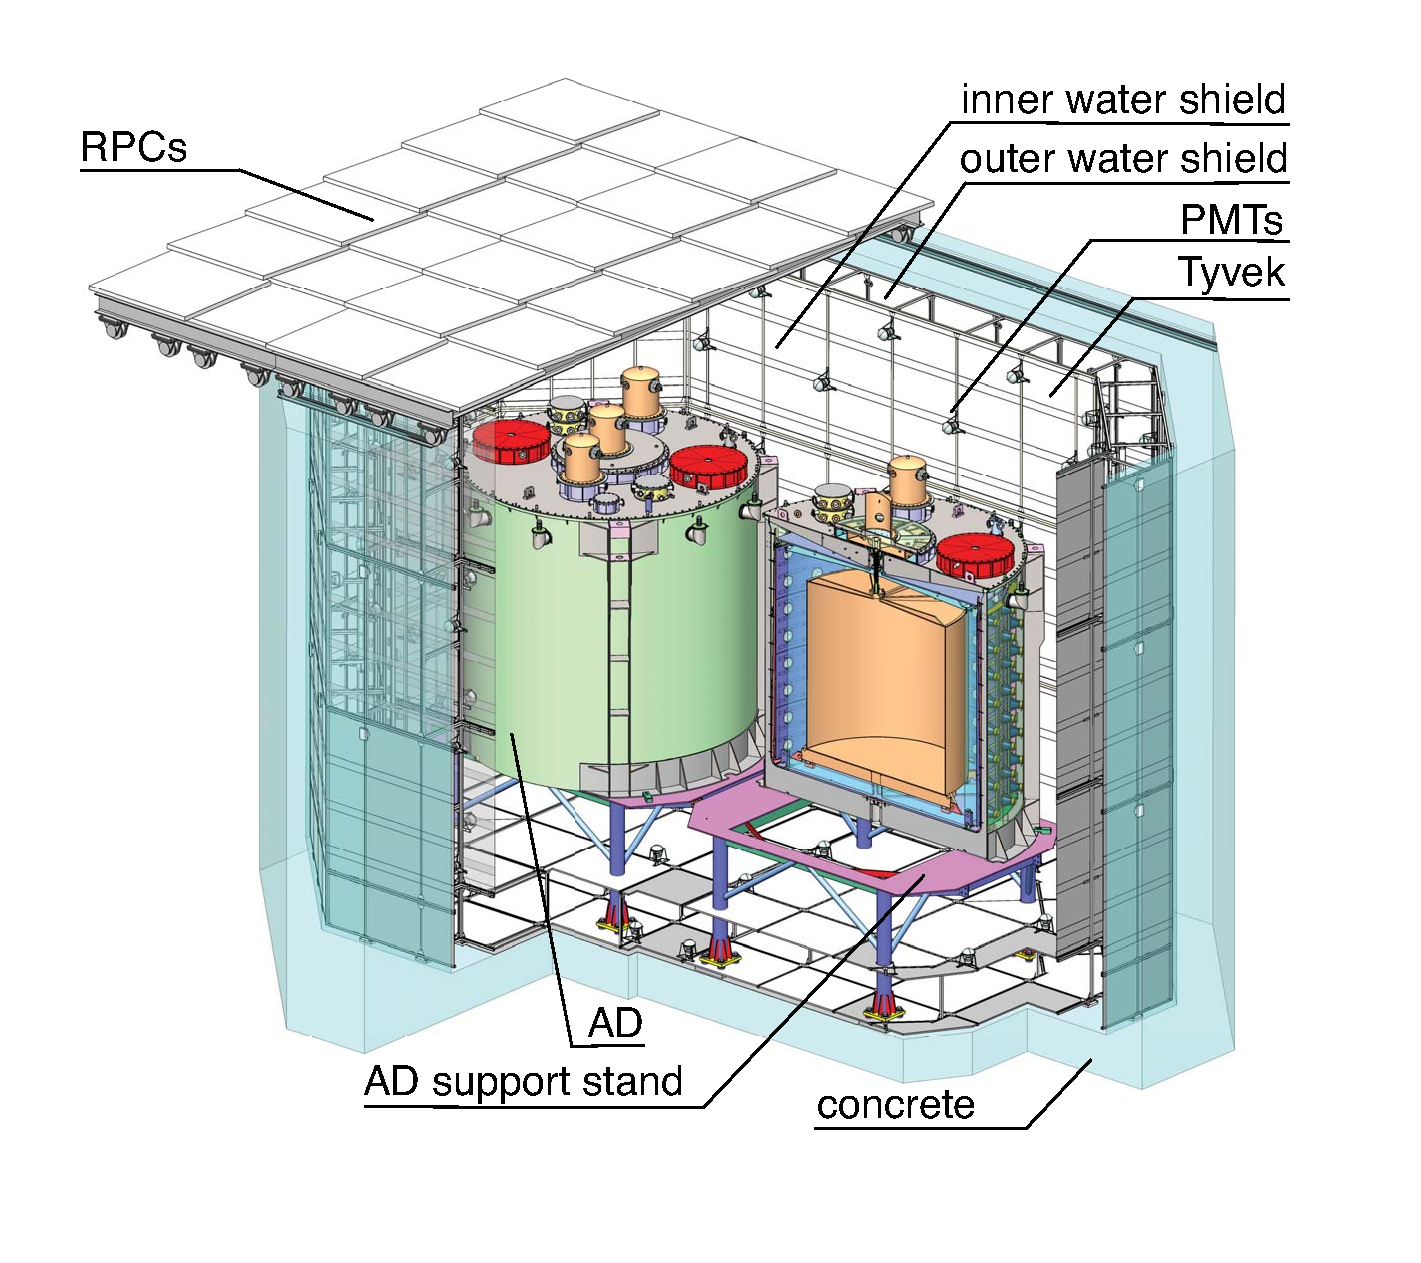
\includegraphics[scale=0.4]{exp_near_site_diagram.pdf}
  \caption{Water pool (including ADs) as configured in the near halls. The far
    hall is similar, with four ADs instead of two. From \cite{An_2017}.}
  \label{fig:expPool}
\end{figure}

Within each experimental hall, the ADs are immersed together inside an
instrumented pool of ultra-pure water. The water pools serve two purposes:
First, to shield the ADs against both ambient $\gamma$ radioactivity and
muon-induced rock neutrons, and second, to detect atmospheric muons that pass
within the vicinity of the ADs. With respect to shielding, the $\sim$2.5~m-thick
layer of water surrounding the ADs (in all directions) reduced the $\gamma$ and
neutron event rate by a factor of $10^6$; without this suppression, antineutrino
detection would be impossible.

Meanwhile, muon detection was accomplished by using PMTs\footnote{The water pool
  PMTs consisted of 619 Hamamatsu R5912 PMTs, as used in the ADs, as well as 341
  EMI 9350KA and D642KB PMTs recycled from the MACRO experiment. The MACRO PMTs
  ultimately proved to be somewhat failure-prone, but not to the point of
  degrading the overall muon detection efficiency.} to observe the Cerenkov
light produced when muons traverse the water. In order to allow for
cross-checking of the muon system \cite{Hack_2014}, the water pools were divided
by Tyvek sheets into two optically isolated zones, the \emph{inner} and
\emph{outer water pools} (IWP/OWP). The IWP is instrumented by inward-facing
PMTs protruding from the Tyvek, while the OWP is instrumented by both
outward-facing PMTs on the Tyvek and inward-facing PMTs on the walls. The EH1
and EH2 water pools are essentially identical, while the EH3 pool was twice as
wide in order to accommodate four detectors (in a 2x2 arrangement) instead of
two. The FEE and trigger systems for the water pools are the same as those for
the ADs, but the trigger configuration is different: ESUM is not used, and the
NHIT thresholds are $\geq$6 for the IWP and $\ge$7 (8) for the near (far) hall
OWP. Offline, in software, more stringent cuts (e.g., NHIT $\geq$ 12) were used
as the definition of a muon event; AD events were then ignored in the immediate
aftermath of such muons, greatly reducing muon-induced IBD-like backgrounds
(especially neutrons).

Additional muon detection was provided by an assembly of modular resistive plate
chambers (RPCs) mounted on a rolling frame on top of each water pool. Each
module, approximately 2.2~m square and 8~cm thick, contained four layers of
Bakelite sheets instrumented by eight readout strips, oriented alternatingly
(between layers) in the x and y directions. The RPCs thus provide the 2D
coordinate, at around 10~cm resolution, of each muon track that intersects the
RPC plane. Two additional \emph{telescope} modules were installed in each hall
along the center of opposing edges of the water pool, to allow for
high-angular-resolution tracking of a subset of muons in muon-related
studies. The RPCs used HV, FEE, and trigger electronics distinct from those used
by the AD and WP RPCs, with a trigger being issued whenever three out of four
layers in a module are above threshold. Although the RPCs proved to be extremely
useful in studies of muons and muon-induced backgrounds, they are not used in
the analysis described in this thesis, as the water pools alone were sufficient
to detect muons with effectively 100\% efficiency.

\subfilebackmatter

\end{document}
